
\documentclass[12pt, a4paper]{article}
\usepackage{ctex}
\usepackage{graphicx}
\usepackage{booktabs}
\usepackage{geometry}
\usepackage{amsmath}
\geometry{margin=2.5cm}

\title{\textbf{广告点击率多维度分析报告}}
\author{数据分析项目}
\date{2026年11月}

\begin{document}

\maketitle

\section{项目背景}
本报告基于某广告平台的真实投放数据，对用户点击行为进行多维度分析，
探究性别、年龄、产品类别、城市等级等因素对广告点击率（CTR）的影响。

\section{数据说明}
\begin{itemize}
    \item 数据来源：Kaggle广告点击预测数据集
    \item 数据规模：463,291条记录，15个字段
    \item 核心指标：is\_click（1=点击，0=未点击）
    \item 时间范围：2017年7月
\end{itemize}

\section{分析结论}

\subsection{整体点击率}
数据集整体CTR为\textbf{6.76\%}，即每100个看到广告的用户中，
约7人会点击，符合数字广告行业平均水平。

\begin{table}[h]
\centering
\caption{点击行为分布}
\begin{tabular}{lrr}
\toprule
行为 & 人数 & 占比 \\
\midrule
未点击 & 431,960 & 93.24\% \\
点击 & 31,331 & 6.76\% \\
\bottomrule
\end{tabular}
\end{table}

\subsection{性别维度}
\begin{table}[h]
\centering
\caption{各性别点击率}
\begin{tabular}{lr}
\toprule
性别 & 点击率 \\
\midrule
男性 & 6.79\% \\
女性 & 6.44\% \\
\bottomrule
\end{tabular}
\end{table}

男性点击率略高于女性，但差距仅为0.35个百分点，
说明\textbf{性别对点击行为影响不显著}。

\subsection{年龄层维度}
\begin{table}[h]
\centering
\caption{各年龄层点击率}
\begin{tabular}{lr}
\toprule
年龄层 & 点击率 \\
\midrule
0（最年轻） & 8.50\% \\
1 & 7.48\% \\
2 & 7.09\% \\
3 & 6.45\% \\
4 & 5.87\% \\
5 & 7.42\% \\
6（最年长） & 8.23\% \\
\bottomrule
\end{tabular}
\end{table}

年龄层与点击率呈\textbf{U型关系}：最年轻（8.50\%）和最年长（8.23\%）
用户点击率最高，中年用户（4层，5.87\%）点击率最低。
建议广告投放重点关注两端年龄群体。

\subsection{产品类别维度}
\begin{table}[h]
\centering
\caption{各产品类别点击率}
\begin{tabular}{lr}
\toprule
产品类别 & 点击率 \\
\midrule
类别3 & 8.35\% \\
类别1 & 7.16\% \\
类别2 & 6.17\% \\
类别5 & 5.91\% \\
类别4 & 5.89\% \\
\bottomrule
\end{tabular}
\end{table}

类别3点击率最高（8.35\%），比最低的类别4（5.89\%）\textbf{高出42\%}，
说明产品类别是影响CTR的重要因素。

\subsection{城市等级维度}
各城市等级点击率介于6.53\%至6.98\%之间，差距极小，
说明\textbf{城市发展等级对点击行为影响不大}。

\section{可视化图表}
\begin{figure}[h]
\centering
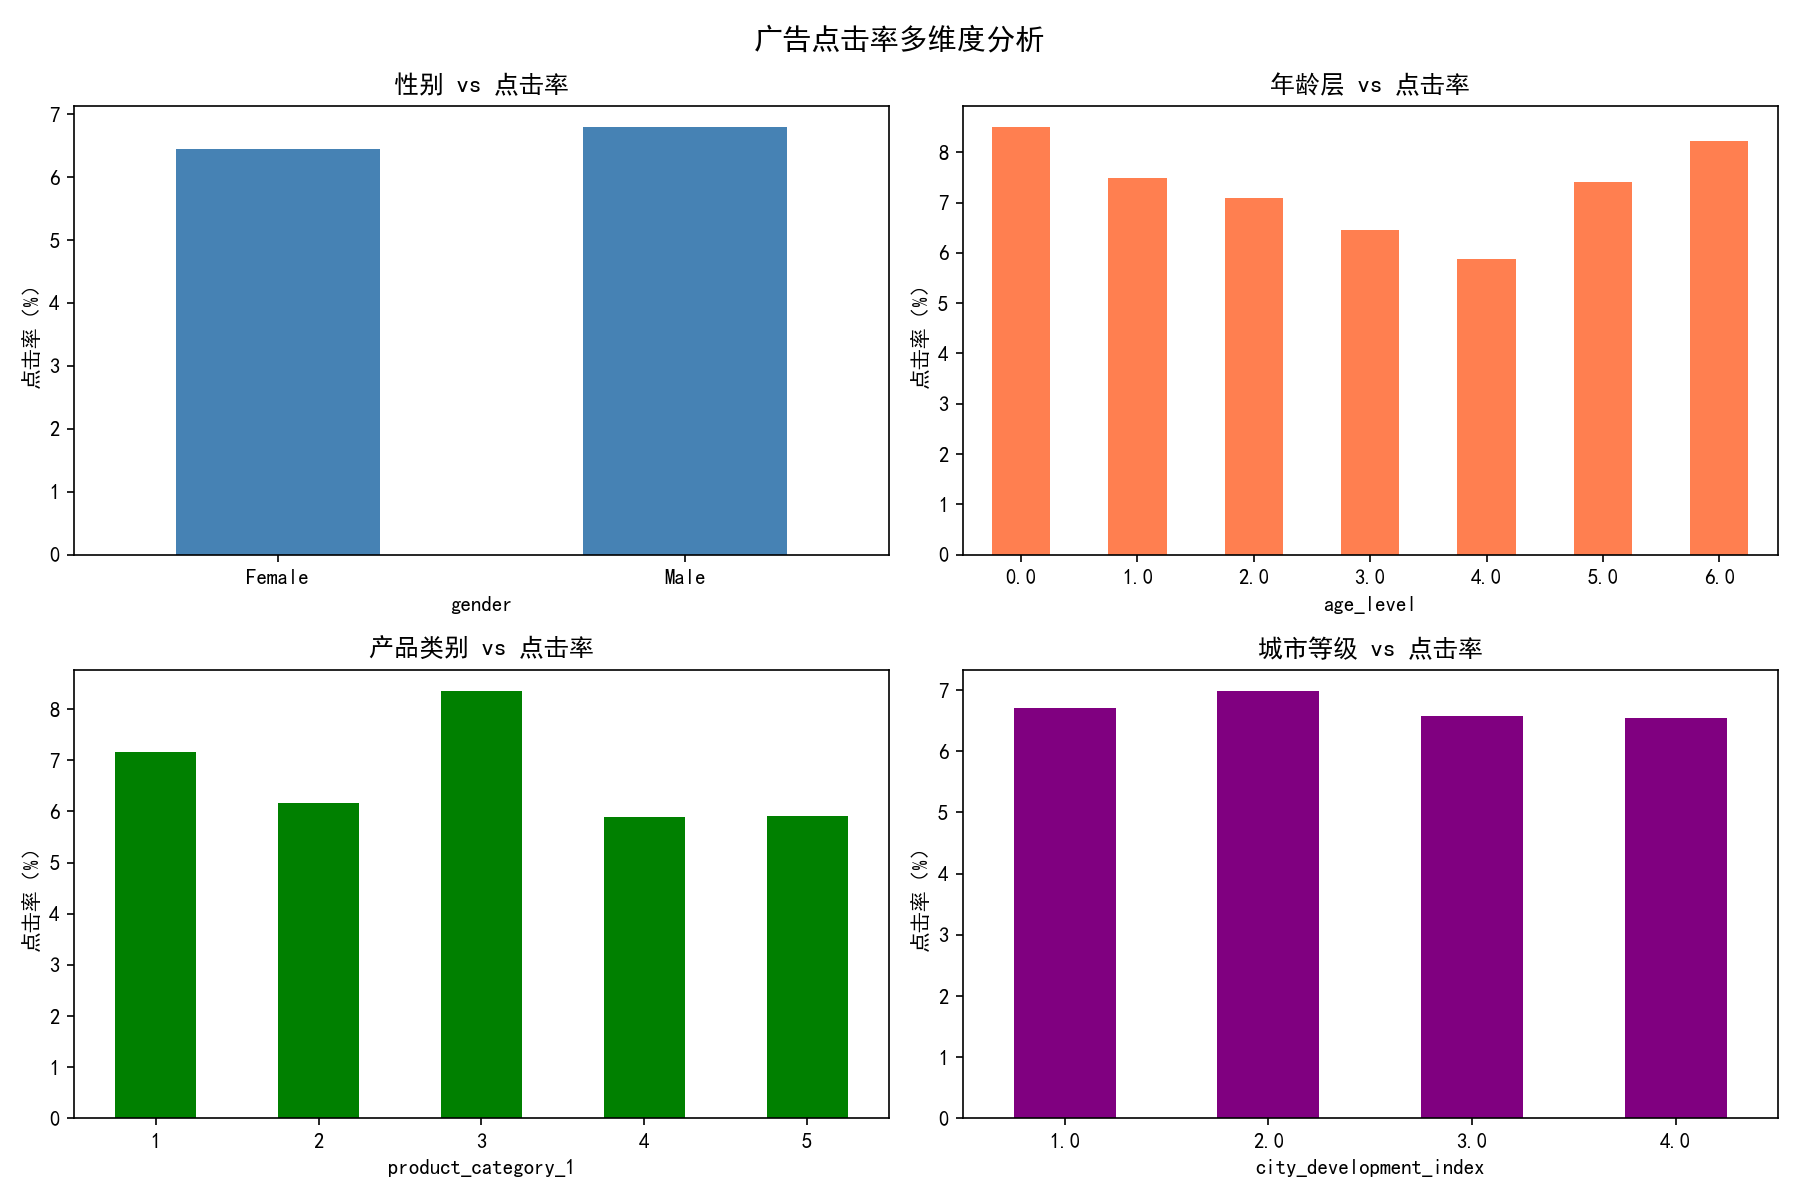
\includegraphics[width=0.9\textwidth]{ad_ctr_analysis_charts.png}
\caption{广告点击率多维度分析图表}
\end{figure}
\section{深度交叉分析}

\subsection{性别与年龄层的交叉点击率}
通过透视表对性别与年龄层进行交叉分析，发现单维度分析中被掩盖的规律。

\begin{figure}[h]
\centering
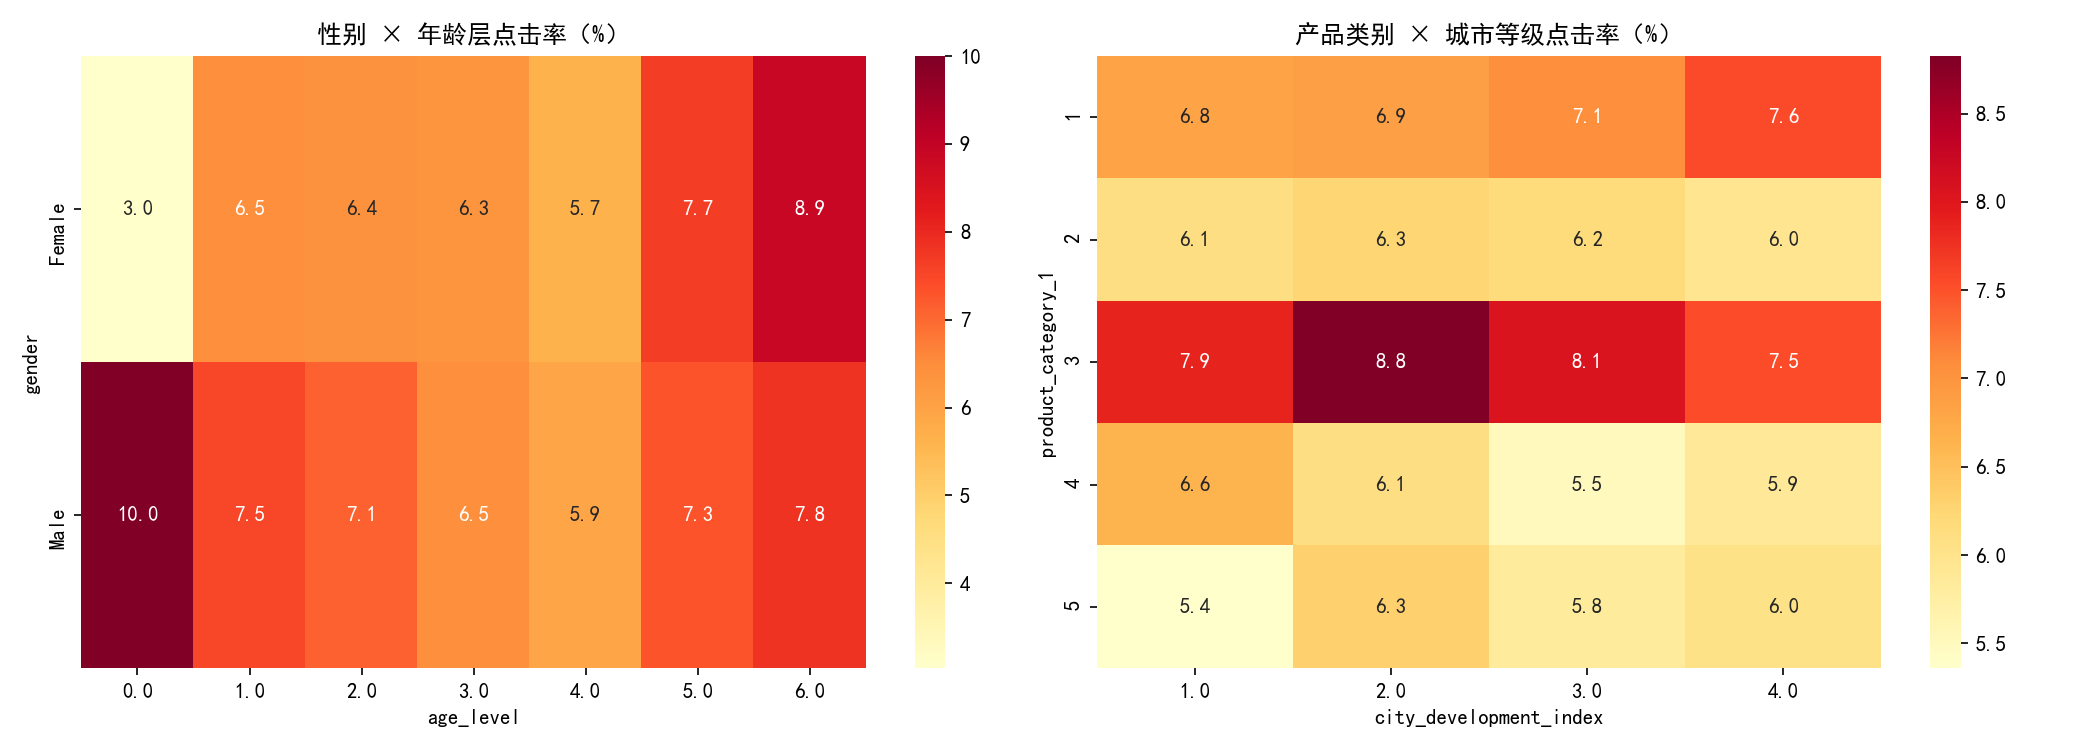
\includegraphics[width=0.9\textwidth]{pivot_heatmap.png}
\caption{透视表热力图：性别×年龄层 与 产品类别×城市等级}
\end{figure}

\textbf{主要发现：}
\begin{itemize}
    \item 年轻男性（年龄层0）点击率高达\textbf{10.00\%}，是整体均值6.76\%的1.5倍，
    是最高价值广告受众
    \item 年轻女性（年龄层0）点击率仅3.03\%，与年轻男性差距悬殊，
    说明针对年轻用户的广告需区分性别投放
    \item 年长女性（年龄层6）点击率达8.89\%，高于年长男性（7.83\%），
    两性在高年龄层呈现反转规律
\end{itemize}

\subsection{产品类别与城市等级的交叉点击率}
\textbf{主要发现：}
\begin{itemize}
    \item 产品类别3在城市等级2表现最强，点击率达\textbf{8.83\%}，
    建议重点在二线城市投放类别3广告
    \item 产品类别1呈现城市等级越高点击率越高的规律
    （1.0城市6.83\% → 4.0城市7.56\%），适合高线城市投放
    \item 产品类别4在所有城市等级表现均差，建议重新评估该类别广告策略
\end{itemize}

\section{总结}
\begin{itemize}
    \item 整体CTR为6.76\%，符合行业正常水平
    \item 性别和城市等级单独来看对点击率影响不显著
    \item 年龄与点击率呈U型关系，两端年龄群体更易点击
    \item 产品类别3效果最佳（8.35\%），比最差类别4高出42\%
    \item 交叉分析发现：年轻男性CTR达10\%，是最高价值广告受众
    \item 产品类别3在二线城市（等级2）表现最强，达8.83\%
    \item 建议广告投放优先针对年轻男性和年长女性，重点推广类别3产品
\end{itemize}

\end{document}
